This section includes Alloy code that describes the model and checks wether it is consistent or not.
At the end of the code, Class Diagram and Alloy generated World are shown.

\myparagraph{Alloy Code}
% Settings for Alloy code listing.
\lstset{
    language=alloy,
    numbers=left,
    numberstyle=\tiny,
    stepnumber=2,
    tabsize=4,
    keywordstyle=\color{alloy-keyword}\bfseries,
    commentstyle=\color{alloy-comment},
    stringstyle=\color{alloy-string},
    basicstyle=\small\fontfamily{pcr}\selectfont, % Courier font family
}

% Includes the Alloy model file.
\lstinputlisting{./files/Alloy.als}
\vfill

\vspace{1cm}

Following are Alloy execution results: \\ \\

   Executing "Run specialUsersCanMakeMoreThanOneDataRequest" \\ \noindent
      Solver=sat4j Bitwidth=4 MaxSeq=4 SkolemDepth=1 Symmetry=20
      16579 vars. 1521 primary vars. 41961 clauses. 73ms. \\ \noindent
      Instance found. Predicate is consistent. 110ms.

   \vspace{1cm}

   Executing "Run usersCanPartecipateInMoreThanOneRun" \\ \noindent
      Solver=sat4j Bitwidth=4 MaxSeq=4 SkolemDepth=1 Symmetry=20
      16579 vars. 1521 primary vars. 41961 clauses. 71ms. \\ \noindent
      Instance found. Predicate is consistent. 98ms.

   \vspace{1cm}

   Executing "Check noLessThan1000UsersInGroupDataRequests" \\ \noindent
      Solver=sat4j Bitwidth=4 MaxSeq=4 SkolemDepth=1 Symmetry=20
      0 vars. 0 primary vars. 0 clauses. 70ms. \\ \noindent
      No counterexample found. Assertion may be valid. 0ms.

   \vspace{1cm}

   Executing "Check noPaymentForNotAcceptedSingleUserDataRequests" \\ \noindent
      Solver=sat4j Bitwidth=4 MaxSeq=4 SkolemDepth=1 Symmetry=20
      16562 vars. 1521 primary vars. 41896 clauses. 97ms. \\ \noindent
      No counterexample found. Assertion may be valid. 18ms.

   \vspace{1cm}

   Executing "Check noSOSCallWithoutBadStatus" \\ \noindent
      Solver=sat4j Bitwidth=4 MaxSeq=4 SkolemDepth=1 Symmetry=20
      16776 vars. 1521 primary vars. 42909 clauses. 72ms. \\ \noindent
      No counterexample found. Assertion may be valid. 29ms.

   \vspace{1cm}

   Executing "Check noGroupRequestsMoreThan1000UsersNotAccepted" \\ \noindent
      Solver=sat4j Bitwidth=4 MaxSeq=4 SkolemDepth=1 Symmetry=20
      0 vars. 0 primary vars. 0 clauses. 50ms. \\ \noindent
      No counterexample found. Assertion may be valid. 1ms.

   \vspace{1cm}

   Executing "Check noSavedAddressesNotUsed" \\ \noindent
      Solver=sat4j Bitwidth=4 MaxSeq=4 SkolemDepth=1 Symmetry=20
      16454 vars. 1524 primary vars. 41696 clauses. 48ms. \\ \noindent
      No counterexample found. Assertion may be valid. 11ms.

   \vspace{1cm}

   Executing "Check noPaymentBeforeRequest" \\ \noindent
      Solver=sat4j Bitwidth=4 MaxSeq=4 SkolemDepth=1 Symmetry=20
      16973 vars. 1521 primary vars. 43394 clauses. 67ms. \\ \noindent
      No counterexample found. Assertion may be valid. 74ms.

   \vspace{1cm}

   Executing "Check noDownloadBeforeRequestAcceptedAndPaid" \\ \noindent
      Solver=sat4j Bitwidth=4 MaxSeq=4 SkolemDepth=1 Symmetry=20
      16629 vars. 1521 primary vars. 42008 clauses. 61ms. \\ \noindent
      No counterexample found. Assertion may be valid. 37ms.

   \vspace{1cm}

   Executing "Check noDeviceIsWorkingIfSmartphoneHasEmptyBattery" \\ \noindent
      Solver=sat4j Bitwidth=4 MaxSeq=4 SkolemDepth=1 Symmetry=20
      16581 vars. 1521 primary vars. 41928 clauses. 71ms. \\ \noindent
      No counterexample found. Assertion may be valid. 10ms.

   \vspace{1cm}

   Executing "Check noHealthStatusMaxPressureLowerThanMinPressure" \\ \noindent
      Solver=sat4j Bitwidth=4 MaxSeq=4 SkolemDepth=1 Symmetry=20
      16803 vars. 1518 primary vars. 43084 clauses. 65ms. \\ \noindent
      No counterexample found. Assertion may be valid. 65ms.

   \vspace{1cm}

   Executing "Check noGoodHealthStatusWithBadValues" \\ \noindent
      Solver=sat4j Bitwidth=4 MaxSeq=4 SkolemDepth=1 Symmetry=20
      0 vars. 0 primary vars. 0 clauses. 52ms. \\ \noindent
      No counterexample found. Assertion may be valid. 0ms.

   \vspace{1cm}

   Executing "Check noBadHealthStatusWithGoodValues" \\ \noindent
      Solver=sat4j Bitwidth=4 MaxSeq=4 SkolemDepth=1 Symmetry=20
      0 vars. 0 primary vars. 0 clauses. 48ms. \\ \noindent
      No counterexample found. Assertion may be valid. 1ms.

   \vspace{1cm}

   Executing "Check noRegistrationAfterDeadline" \\ \noindent
      Solver=sat4j Bitwidth=4 MaxSeq=4 SkolemDepth=1 Symmetry=20
      16973 vars. 1521 primary vars. 43394 clauses. 58ms. \\ \noindent
      No counterexample found. Assertion may be valid. 57ms.

   \vspace{1cm}

   Executing "Check noHealthStatusRecordWithoutDevice" \\ \noindent
      Solver=sat4j Bitwidth=4 MaxSeq=4 SkolemDepth=1 Symmetry=20
      16532 vars. 1518 primary vars. 41848 clauses. 47ms. \\ \noindent
      No counterexample found. Assertion may be valid. 30ms.

   \vspace{1cm}

   Executing "Check noPositionRecordWithoutSmartphone" \\ \noindent
      Solver=sat4j Bitwidth=4 MaxSeq=4 SkolemDepth=1 Symmetry=20
      16532 vars. 1518 primary vars. 41848 clauses. 55ms. \\ \noindent
      No counterexample found. Assertion may be valid. 20ms.

   \vspace{1cm}

   Executing "Check noPaymentWithoutDataRequest" \\ \noindent
      Solver=sat4j Bitwidth=4 MaxSeq=4 SkolemDepth=1 Symmetry=20
      16532 vars. 1518 primary vars. 41848 clauses. 40ms. \\ \noindent
      No counterexample found. Assertion may be valid. 6ms.

   \vspace{1cm}

   Executing "Check noSmartphoneWithoutUser" \\ \noindent
      Solver=sat4j Bitwidth=4 MaxSeq=4 SkolemDepth=1 Symmetry=20
      16532 vars. 1518 primary vars. 41848 clauses. 68ms. \\ \noindent
      No counterexample found. Assertion may be valid. 36ms.

   \vspace{1cm}

   Executing "Check noSOSCallWithoutSmartphone" \\ \noindent
      Solver=sat4j Bitwidth=4 MaxSeq=4 SkolemDepth=1 Symmetry=20
      16532 vars. 1518 primary vars. 41848 clauses. 57ms. \\ \noindent
      No counterexample found. Assertion may be valid. 7ms.

   \vspace{1cm}

   Executing "Check noDeviceWithoutSmartphone" \\ \noindent
      Solver=sat4j Bitwidth=4 MaxSeq=4 SkolemDepth=1 Symmetry=20
      16532 vars. 1518 primary vars. 41848 clauses. 42ms. \\ \noindent
      No counterexample found. Assertion may be valid. 5ms.

   \vspace{1cm}

   Executing "Check noPositionWithoutRunOrPositionRecord" \\ \noindent
      Solver=sat4j Bitwidth=4 MaxSeq=4 SkolemDepth=1 Symmetry=20
      16583 vars. 1518 primary vars. 41932 clauses. 52ms. \\ \noindent
      No counterexample found. Assertion may be valid. 30ms.

   \vspace{1cm}

   Executing "Check noTwoRegSameUserSameRun" \\ \noindent
      Solver=sat4j Bitwidth=4 MaxSeq=4 SkolemDepth=1 Symmetry=20
      16613 vars. 1521 primary vars. 42055 clauses. 42ms. \\ \noindent
      No counterexample found. Assertion may be valid. 16ms.

   \vspace{1cm}

   Executing "Run show" \\ \noindent
      Solver=sat4j Bitwidth=4 MaxSeq=4 SkolemDepth=1 Symmetry=20
      16493 vars. 1515 primary vars. 41785 clauses. 53ms. \\ \noindent
      Instance found. Predicate is consistent. 78ms.

   \vspace{1cm}

   \begin{figure}[H]
   \begin{center}
     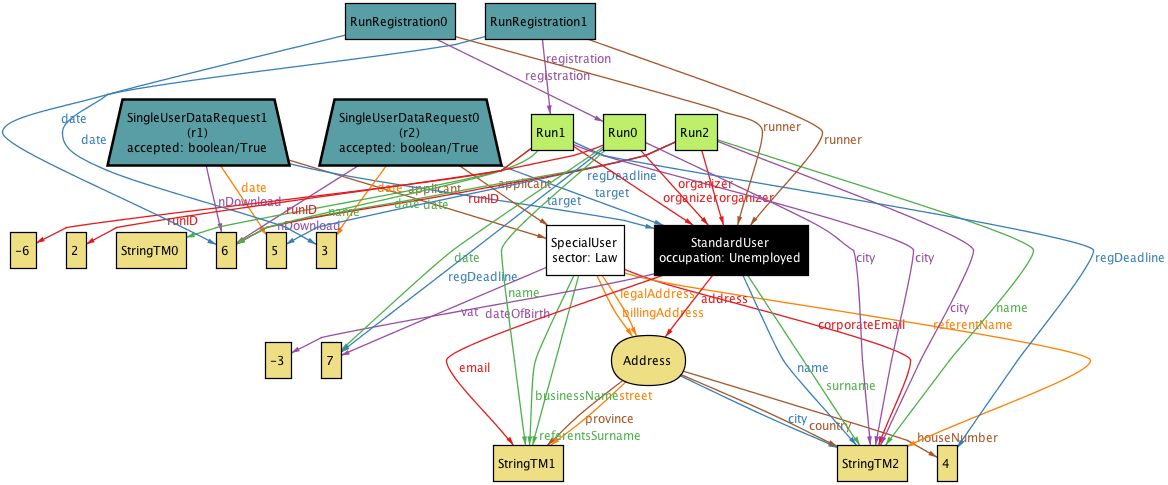
\includegraphics[width=0.80\paperwidth]{./img/alloy/alloy2.png}
     \hspace{0.05\linewidth}
     \centering
     \caption{An example of \textit{Generated World}}
     \label{img:generatedWorld}
   \end{center}
   \end{figure}

 \begin{figure}[H]
 \begin{center}
   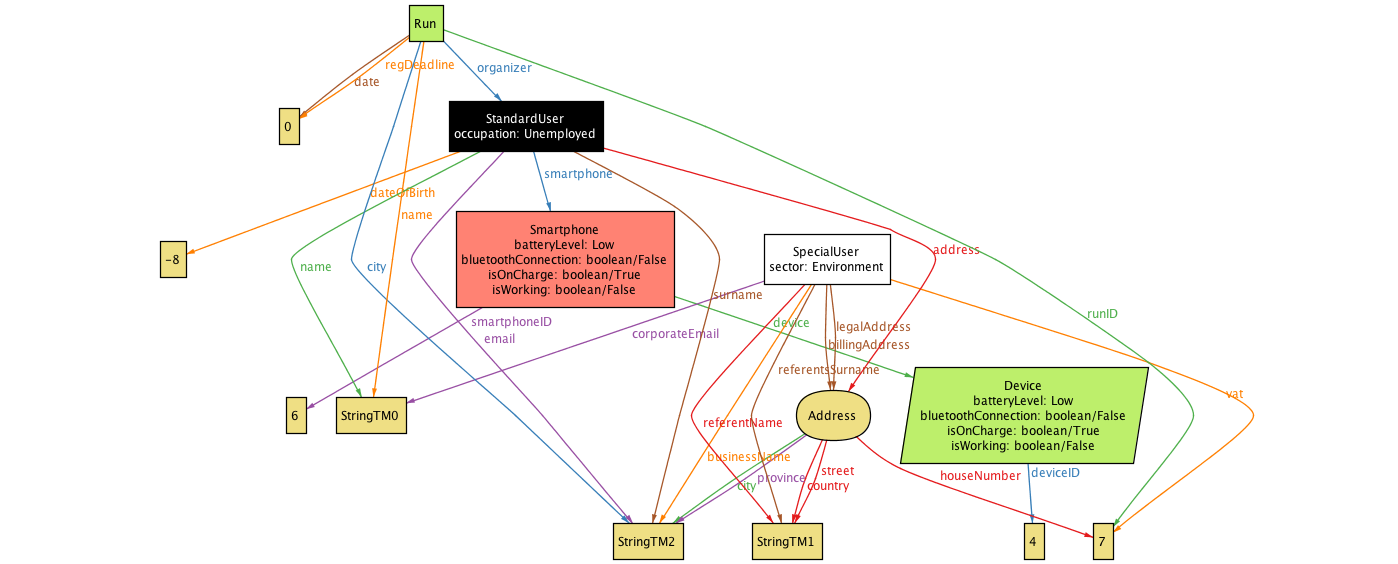
\includegraphics[width=0.80\paperwidth]{./img/alloy/alloy3.png}
   \hspace{0.05\linewidth}
   \centering
   \caption{An other example of \textit{Generated World}}
   \label{img:generatedWorld}
 \end{center}
 \end{figure}

 \begin{figure}[H]
 \begin{center}
   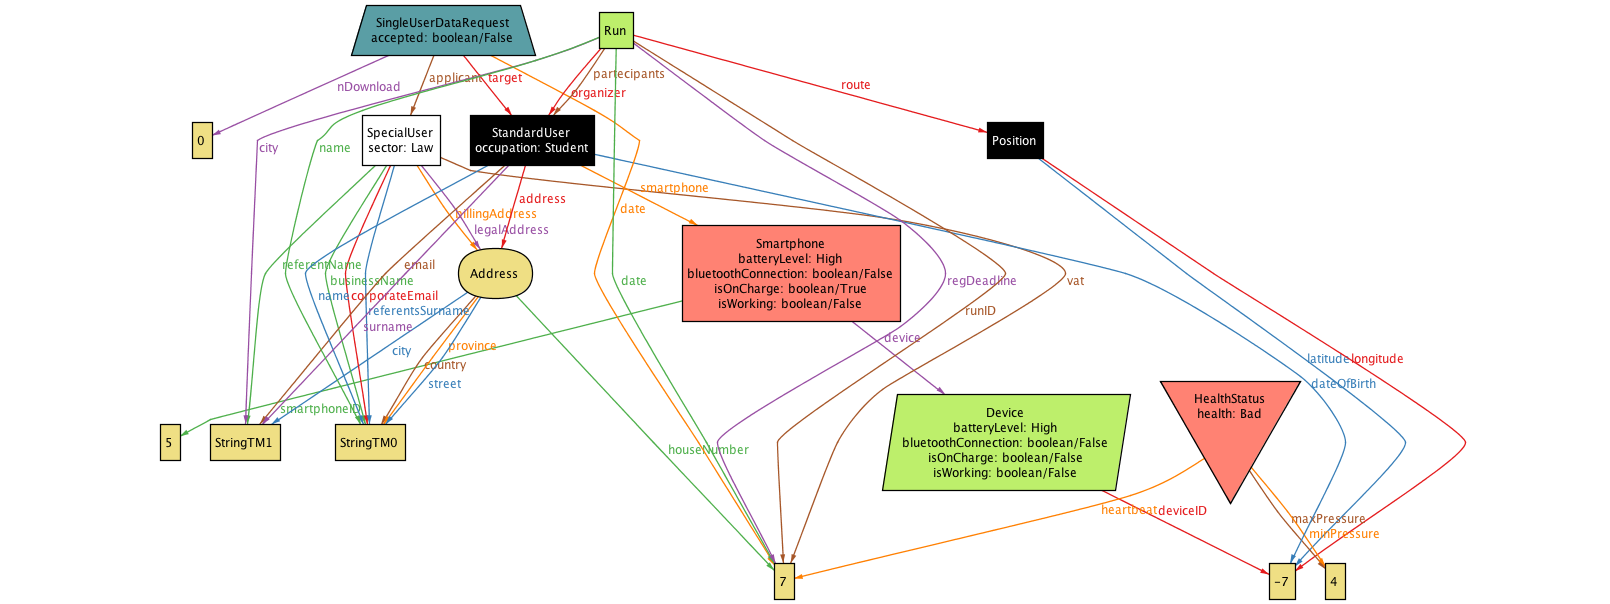
\includegraphics[width=0.80\paperwidth]{./img/alloy/alloy5.png}
   \hspace{0.05\linewidth}
   \centering
   \caption{An other example of \textit{Generated World}}
   \label{img:generatedWorld}
 \end{center}
 \end{figure}

 \begin{figure}[H]
 \begin{center}
   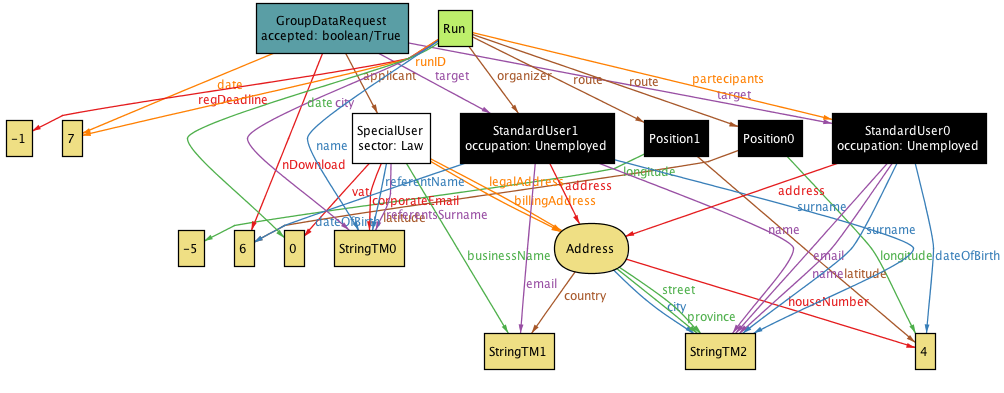
\includegraphics[width=0.80\paperwidth]{./img/alloy/alloy6.png}
   \hspace{0.05\linewidth}
   \centering
   \caption{An other example of \textit{Generated World}. In this case in order to generate this World, due to computational and representation problems, the minimum number of Standard Users allowed for group data request has been changed from 1000 to 2.}
   \label{img:generatedWorld}
 \end{center}
 \end{figure}


\vspace{1cm}

\begin{figure}[H]
  \begin{center}
  	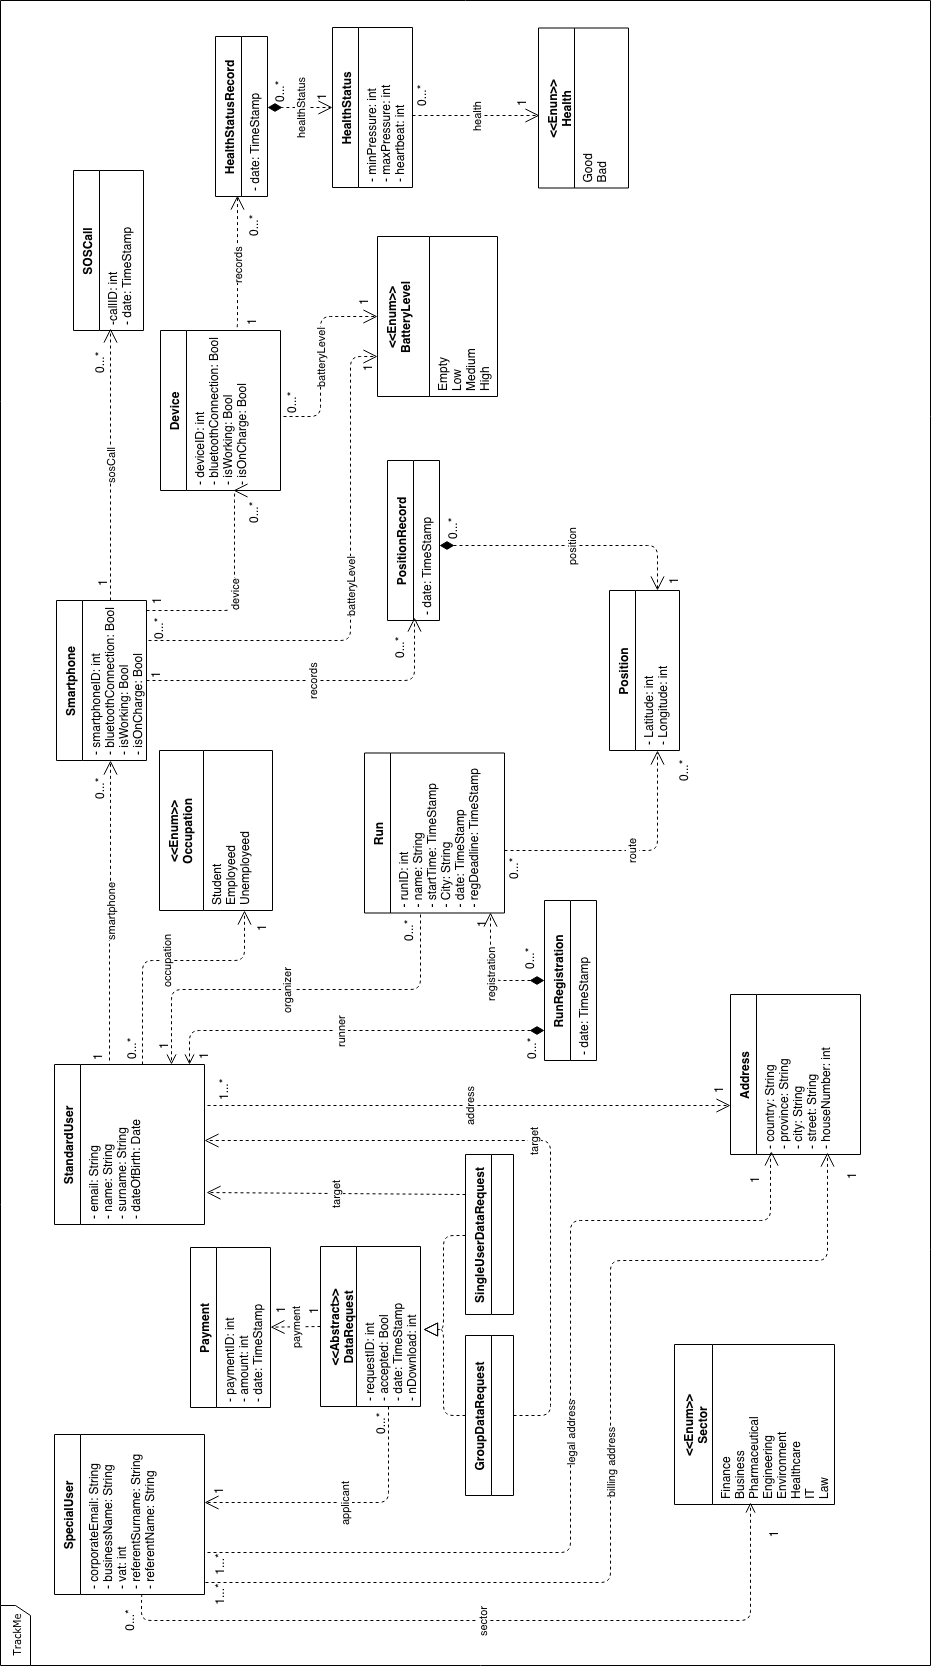
\includegraphics[height=0.68\paperheight]{./img/Class_Diagram.png}
		\caption{\textit{Class diagram} of the structure of the system-to-be.}
    \hspace{0.05\linewidth}
    \centering
		\label{classDiagram}
    \end{center}
\end{figure}
